	%
% LaTeX template for Student Thesis & PhD Thesis
%
% Institute of Biomedical Engineering
% Karlsruhe Institute of Technology (KIT)
% www.ibt.kit.edu
%
% IBT template v2.8.1 (2014-05-17)
% Last changes by js908 
%


%%%%%%%%%%%%%%%%%%%%%%%%%%%%%%%%%%%%%%%%%%%%%%%%%%%%%%
% ATTENTION: In this template, do NOT use underscores ("_") in labels, figure file names etc., because this will produce errors!
% Alternatively: Look at the "Hack" in LaTeXdefs.tex, but use it at your own risk!
%%%%%%%%%%%%%%%%%%%%%%%%%%%%%%%%%%%%%%%%%%%%%%%%%%%%%%



%%%%%%%%%%%%%%%%%%%
% Document Definitions %
%%%%%%%%%%%%%%%%%%%
% (Based on http://cupnet.net/latex-conditions/)

%%% Language of thesis
\newif\ifenglish
\englishtrue 				% define if thesis is in English
%\englishfalse 					% define if thesis is in German

%%% APA style citations
\newif\ifapa
\apatrue 						% define if APA style references are desired
%\apafalse 						% define if IEEE style references are desired

%%% PhD Thesis or Student Thesis
\newif\ifthesisisdiss
%\thesisisdisstrue 			% define for PhD Thesis
\thesisisdissfalse 			% define for Student Thesis

%%% PhD Thesis for preparation or book print
\newif\ifdissforprint
%\dissforprinttrue 			% define for PhD Thesis for Print Process at KIT Scientific Publishing
\dissforprintfalse 			% define for PhD Thesis for regular A4 printout

%%%%%%%%%%%%%%%%%%%%%%
% Document Definitions  END%
%%%%%%%%%%%%%%%%%%%%%%



%%%%%%%%%%%%%%%%%%
%%% LaTeX matters %%%
%%%%%%%%%%%%%%%%%%

\documentclass[envcountsame,envcountchap,twoside,a4paper]{styles/svmono}


%%%%%%%%%%%%%%%%%%%%%%%
% For KIT border on title page %
%%%%%%%%%%%%%%%%%%%%%%%
%\usepackage[absolute,overlay]{textpos}
%\usepackage{tikz}



%%%%%%%%%%%%%%%%%%%
% Extensions for Tables  %
%%%%%%%%%%%%%%%%%%%
%% an example of a colored table can be found "kapitel5.tex"
\usepackage{color}
\usepackage{colortbl}
\definecolor{hellgrau}{rgb}{0.95,0.95,0.95}
\definecolor{hellblau}{rgb}{0.76,0.92,1}
\definecolor{hellgrun}{cmyk}{0.8,0,1,0}
\definecolor{hellgelb}{rgb}{0.99,0.99,0.81}
%% END color-tables
\usepackage{multicol} 							% for \multicol command in tables
%\usepackage{threeparttable} 				% enables to add footnotes into tables
%

 \renewcommand{\sfdefault}{phv}
% \usepackage[pdf]{pstricks}
%\usepackage[crop=off]{auto-pst-pdf}
\usepackage{pstool}
\usepackage{psfrag}


%%%%%%%%%%%%%%%
% General Package %
%%%%%%%%%%%%%%%
\ifdissforprint
	\usepackage{styles/diplDissPrint}
\else
	\usepackage{styles/dipl}
\fi
\ifenglish
	\shortindexingoff
	\usepackage[english]{babel}			% Uncomment for ENGLISH figure captions etc.	
	\shortindexingon
\fi
\graphicspath{{pics/}} 							% defines path where figures are stored



%%%%%%%%%%%%%%%%%%%%%%%%%%%%%%%
% Necessary Packages for this Template  %
%%%%%%%%%%%%%%%%%%%%%%%%%%%%%%%
%\usepackage{graphicx} 							% figure environment
%\usepackage{epsfig}								% allows to directly embed eps figures when using pdflatex
\usepackage{subfigure} 							% enables the use of subfigure 
%\usepackage[
%  unicode=true,
%  a4paper=true,
%  pdfpagelabels=true,
%  pdfborder={0 0 0},
%  plainpages=false,
%  pdftitle={Title of your work}, 				% FILL IN YOUR DATA HERE !
%  pdfauthor={Your name},
%  pdfsubject={Diplomarbeit},
%  pdfkeywords={keyword1, keyword2,keyword2},
%  pdfstartpage=1,
%  pdftex,          										% alternatives: ps2pdf, dvips, latex2html
%]{hyperref}
\ifthesisisdiss
	\RequirePackage{times,mathptmx} 		% activate this for a PhD thesis
\fi


%%%%%%%%%%%%%%%%
% Citation Style 1/2 %
%%%%%%%%%%%%%%%%
%%% APA Style (name, year in brackets) %%%
%% uncomment the following two lines to enable APA-style references:
\ifapa
	\usepackage[square]{natbib}
	\renewcommand{\cite}{\citep}
	% you also need to change the bibliographystyle from {dipl} to {natbib} (see end of document)
	% Before compiling the document with the new style, clean up LaTeX file, as otherwise you will encount errors
\else
	%%% IEEE style (numbers in brackets) %%%
	\usepackage[numbers,sort&compress]{natbib} % to sort references in alphabetical oder at end and in ascending oder in text and use "-" instead of multiple "..,..,..," in the text
\fi


%%%%%%%%%%
% \bibentry %
%%%%%%%%%%
%% uncomment the next to lines for the command \bibentry
%% the command is useful for a list of publications in a PhD thesis
% \usepackage{bibentry}
% \nobibliography*


%%%%%%%%%%%%%%%%%%%%%%%
% Other Interesting Packages  %
%%%%%%%%%%%%%%%%%%%%%%%
%% Some packages that might be interesting
%\RequirePackage{mathcomp} 							% provides \tcmu, \tcomega
%\RequirePackage{overpic}  								% overlay images with other images,
                          												% e.g. scale or legend
%\usepackage[novbox]{pdfsync}     						% allow linking back from PDF to position
                          												% in source code when using TeXShop 
%\usepackage[normalem]{ulem} 							% for command \sout = strike out
%\usepackage[framed,autolinebreaks]{styles/mcode} 	% to include Matlab source code into LaTeX
%\usepackage{rotating}  									% if you want to rotate tables, pages, figures to landscape


%%%%%%%%%%%%%%%%%%%%
% Workaround for "_" bug %
%%%%%%%%%%%%%%%%%%%%
% This "hack" was not fully tested with the template.
% Use at your own risk!
% Uncomment this if you want to use colored tables:
% begingroup
%   \catcode`\_=\active
%   \gdef_#1{\ensuremath{\sb{\mathrm{#1}}}}
% \endgroup
% \mathcode`\_=\string"8000
% \catcode`\_=12  
% END underscore-hack (leave this line commented)


%%%%%%%%%%%%%%%%%%%%%%%%%%%%%%
% Short definitions for trademarks etc.  %
%%%%%%%%%%%%%%%%%%%%%%%%%%%%%%
\def\TReg{\textsuperscript{\textregistered}}
\def\TCop{\textsuperscript{\textcopyright}}
\def\TTra{\textsuperscript{\texttrademark}}


%%%%%%%%%%%%%%%%%%%%%%%%%%%%%%%%%%
% Define hyphenation (Silbentrennung) here  %
%%%%%%%%%%%%%%%%%%%%%%%%%%%%%%%%%%
\hyphenation{set-up electro-physiology}

 				% Definitions for packages, commands, hyphenation etc.

\hyphenation{Li-te-ra-tur-ver-zeich-nis}

\begin{document}
\pagenumbering{alph}



%%%%%%%%%%%%%%
%%% Title Page %%%
%%%%%%%%%%%%%%

\ifthesisisdiss
	\begin{titlepage}
 \parindent0cm
\begin{center}

\begin{minipage}[c]{16.5cm}
\begin{center}
   {\LARGE
   \begin{bf}
   \hspace{-1cm}
     Dies ist der Titel Deiner Arbeit,\\
   \hspace{-1cm}
     der sich z.~B. auch \"uber mehrere\\
   \hspace{-1cm}
      Zeilen verteilen kann.\\
    \end{bf}
	}
\end{center}
\end{minipage}

    \vspace{2.5cm}
    {\large Zur Erlangung des akademischen Grades eines}\\
    
    \vspace{1.2cm}
     {\Large DOKTOR-INGENIEURS}\\
    \vspace{1.2cm}
    \ifdissforprint
   		{\large von der Fakult\"at f\"ur}\\ % vor der mündlichen Prüfung: "an" / nach erfolgreichem Abschluss: "von"
   	\else
   		{\large an der Fakult\"at f\"ur}\\ % vor der mündlichen Prüfung: "an" / nach erfolgreichem Abschluss: "von"
   	\fi
    \vspace{0.4cm}
    {\large Elektrotechnik und Informationstechnik}\\
    \vspace{0.4cm}
    {\large des Karlsruher Instituts f\"ur Technologie (KIT) }\\
    \vspace{0.8cm}
    \ifdissforprint
    		{\large genehmigte }\\ % vor der mündlichen Prüfung: "vorgelegte" / nach erfolgreichem Abschluss: "genehmigte"
   	\else
    		{\large vorgelegte }\\ % vor der mündlichen Prüfung: "vorgelegte" / nach erfolgreichem Abschluss: "genehmigte"
   	\fi
    \vspace{1.2cm}
    {\Large DISSERTATION}\\
    \vspace{1.2cm}
    {\large von }\\
    \vspace{0.8cm}
    {\large Dipl.-Ing. <Dein Name>}\\
    \vspace{0.4cm}
    {\large geb. in Musterstadt}\\
    \ifdissforprint
    		 \vspace{2.1cm}
   	\else
    		 \vspace{2.5cm}
   	\fi
   

\begin{large}
\begin{tabular}{l@{\hspace{6mm}}l}
Tag der m\"undlichen Pr\"ufung: & 1. Januar \the\year\\
Referent: & Prof. Dr. rer. nat. Olaf D\"ossel\\
Korreferent: & Prof. Dr. ... \\
\end{tabular}
\end{large}


 \vspace{0.3cm}
  \end{center}
\end{titlepage}

\thispagestyle{empty}
			% Title for PhD thesis
\else
	\begin{titlepage}
 \parindent0cm
   \begin{center}
   \begin{bf}

\begin{minipage}[c]{15.5cm}
\begin{center}
   \begin{huge}
   \hspace{-1cm}
     Removing the effect of respiration\\
    \hspace{-1cm}
     on the heart rate variability\\
   \hspace{-1cm}
     and quantifying the medical impact\\
   \hspace{-1cm}
     of the new uncoupled parameters\\
   \hspace{-1cm}
     when estimating risk of cardiac death\\
   \end {huge}
\end{center}
\end{minipage}

    \vspace{5cm}
    {\Large Master Thesis}\\
    \end{bf}
    
    \vspace{0.5cm}
     {\large presented by}\\
    \vspace{0.5cm}
    \begin{bf}    
     {\Large B.Sc. Michael Kircher}
   \vspace{5cm}
    \end{bf}

\begin{figure}[ht]
 \centering
\includegraphics[width=3.5cm]{KITLOGO}
\end{figure}
 \begin{sc}
 Institut f\"ur Biomedizinische Technik\\
 Prof. Dr. rer. nat. Olaf D\"ossel\\
% Co-Supervisor: Prof. Dr. t.b.a.\\
 Karlsruher Institut f\"ur Technologie\\
\the\year\\
 \end{sc}

 \vspace{0.5cm}
   Supervisor: Gustavo Lenis Parra\\
  \end{center}
\end{titlepage}

\thispagestyle{empty}

\clearemptydoublepage
\newpage
\thispagestyle{empty}

\vspace*{16cm}
{\setlength{\parindent}{0pt}
\textbf{Eidesstattliche Erkl\"arung}\\\\
Hiermit erkl\"are ich an Eides statt, dass ich die vorliegende
Arbeit  selb\-st\"andig  und  ohne  unzul\"assige fremde Hilfsmittel angefertigt habe. W"ortlich oder inhaltlich "ubernommene Stellen sind als solche kenntlich gemacht und die verwendeten Literaturquellen im Literaturverzeichnis  vollst\"andig angegeben. Die \glqq Regeln zur Sicherung guter wissenschaftlicher Praxis im Karlsruher Institut f\"ur Technologie (KIT)\grqq\, in ihrer g"ultigen Form wurden beachtet. 

\vspace{1cm}
{\setlength{\parindent}{0pt}
Karlsruhe, den \the\day.\the\month.\the\year} % this may also be changed to the date of the official end of the thesis
				% Title for student projects
\fi




%%%%%%%%%%%%%%%%%%%%%%%%%%%%%%%%%%%%%%%%%%%%%%%%%%%%%%
\frontmatter %%%%%%%%%%%%%%%%%%%%%%%%%%%%%%%%%%%%%%%%%%%%
%%%%%%%%%%%%%%%%%%%%%%%%%%%%%%%%%%%%%%%%%%%%%%%%%%%%%%

\clearemptydoublepage
\pagenumbering{roman}
\setcounter{page}{1}

\tableofcontents
\newpage\thispagestyle{empty}
\clearemptydoublepage



%%%%%%%%%%%%%%%%%%%%%%%%%%%%%%%%%%%%%%%%%%%%%%%%%%%%%%
\mainmatter %%%%%%%%%%%%%%%%%%%%%%%%%%%%%%%%%%%%%%%%%%%%
%%%%%%%%%%%%%%%%%%%%%%%%%%%%%%%%%%%%%%%%%%%%%%%%%%%%%%

\pagenumbering{arabic}

% switch of document spacing
%\doublespacing 							% = \setstretch{1.6}
%\onehalfspacing 							% = \setstretch{1.3}
%\singlespacing 							% = \setstretch{1.0}

\ifdissforprint
	\setstretch{1.2}							% more line spacing, as in A5 print and font size 13, 1.1 looks too narrow.
\else
	\setstretch{1.1}
\fi



\chapter{Introduction}
\label{introduction}
\thispagestyle{empty}


\newpage\thispagestyle{empty}
\clearemptydoublepage

% Header
%%%%%%%%%%%%%%%%%%%%%%%%%%%%%%%%%%%%%%%%%%%%%%%%%%%%%%%%%%%%%%%%%%%%%%%%%%%%%%%%%%%

\chapter{Fundamentals}
\label{fundamentals}
\thispagestyle{empty}

%%%%%%%%%%%%%%%%%%%%%%%%%%%%%%%%%%%%%%%%%%%%%%%%%%%%%%%%%%%%%%%%%%%%%%%%%%%%%%%%%%%


This chapter includes the most important fundamentals about the cardiac anatomy and physiology, as well as the necessary technical background for understanding the methods developed during the research for this master thesis. The first section covers the human physiology.





% First Section: Physiological Fundamentals
%%%%%%%%%%%%%%%%%%%%%%%%%%%%%%%%%%%%%%%%%%%%%%%%%%%%%%%%%%%%%%%%%%%%%%%%%%%%%%%%%%

\section{Physiological Fundamentals}
\label{physiologicalFundamentals}
Looking at a human heart from an engineer's perspective, it can be described as a highly optimized technical systems. The heart is a strong pump with pipes and valves and it is driven by electric excitation. Just like an artificial system it depends on a control unit, which is able to adapt to different conditions and disturbances. Although the human heart is a very robust and durable system, its efficiency and functionality declines with time. On top the components of this complex system might also fail, if they are exposed to too much stress, again just like in an engineered system. 
In order to detect and possibly solve these failures, the Electrocardiogram (ECG) represents a powerful tool. It is measured using electrodes, which record the electrical excitation on the skin.
\newline
This section describes the most important components of this complex object. It is not intended to give a detailed discourse of the anatomy and physiology, yet the section introduces the necessary facts to understand the analysis methods, developed during the research for this thesis. The topics, which will be introduced, include the heart itself and the Autonomic Nervous System (ANS). The respiratory system and its influence on the functionality of the heart is furthermore described. Subsequently an explanation of the Electrocardiogram (ECG) and its interpretation can be found in the last part of this section.

% Anatomy of the Human Heart
% -----------------------------------------------------------------------------------------------------------------------------------------------------------------------------------------------------------------------
\subsection{The Anatomy and Mechanics of the Human Heart}
\label{anatomy}
\textcolor{green}{
	Here I want to have multiple paragraphs:
	\begin{enumerate}
  		\item location of the heart  
  		\item anatomy of the heart
  		\item blood flow (pulmonary circle,systematic circle,Filling-/Emptying phase)
	\end{enumerate}
}
The human heart is a hollow muscle, which establishes the blood supply to all organs in the body. It is the driving force for the blood circulation in the human body and is located in the thoracic cavity, between the breastbone anteriorly and the backbone posteriorly \cite{sherwood07}. The heart has a broad base on the top directly behind the backbone in the middle of the chest, while the tip of the heart, the apex, is pointed away from the middle to the left. The apex can actually bang against the chest, when the heart beats strongly, which explains the misleading feeling of many, that the heart is located in the left half of the thorax \cite{sherwood07}. The organ resembles a human clenched fist in shape and size and weighs about 250 - 400\,g \cite{schwegler11}, depending on the gender, age and physical fitness of the person. \textcolor{red}{Include a picture to show location of the heart and the reference to the picture here.} 
\newline
The heart consists of two halves, left and right. These two individual halves serve as separate pumps, which are again subdivided into a small chamber, the atrium, and a large chamber, the ventricle. A muscular partition separates the two halves, which is formed by the interatrial septum between the left and right atrium and the interventricular septum between the ventricles.
\begin{figure}
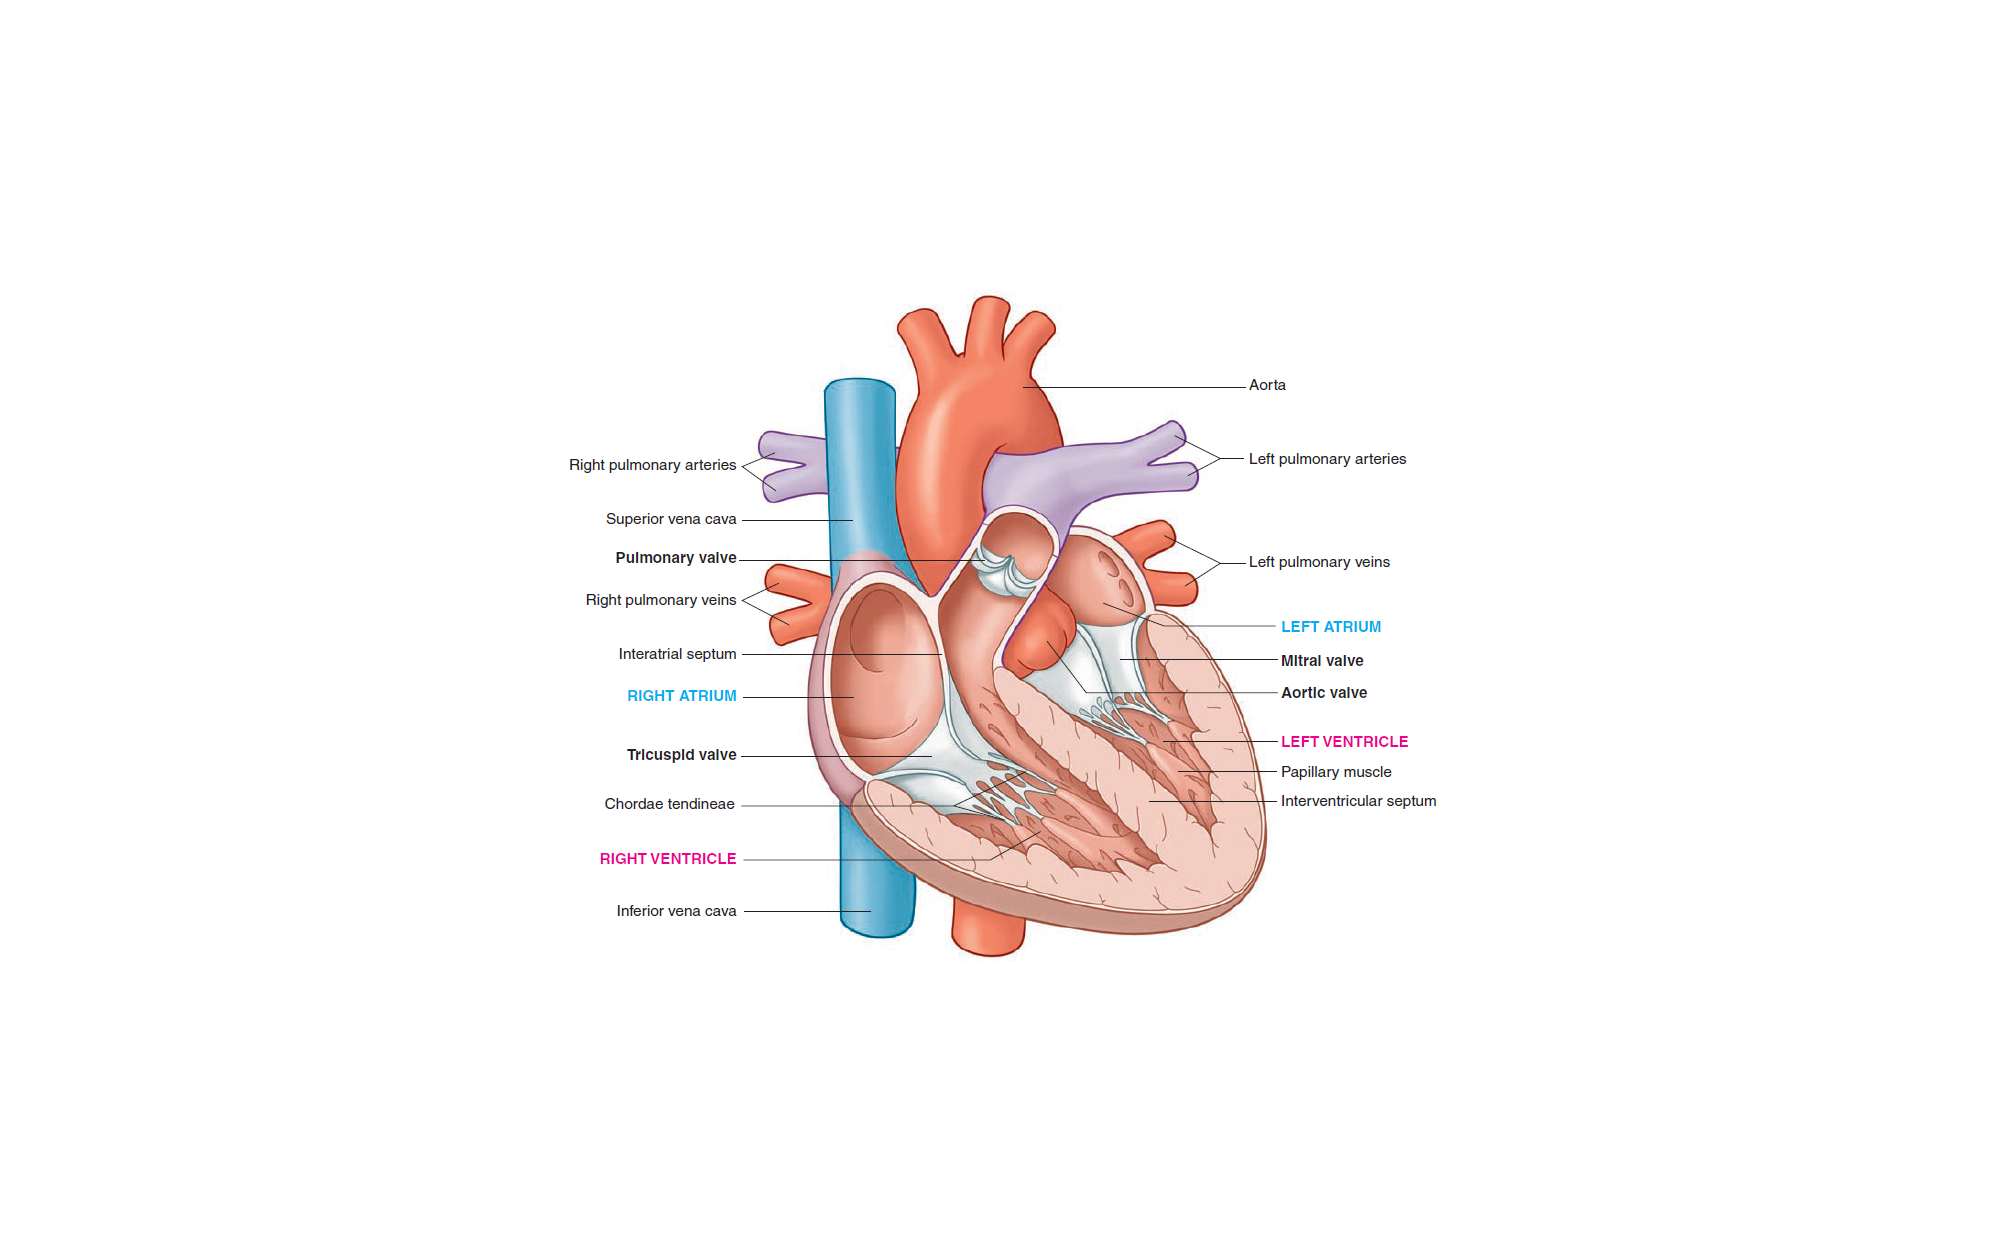
\includegraphics{HeartAnatomy.png}
\end{figure}
\textcolor{red}{Include a picture to show anatomy of the heart and the reference to the picture here.} 
\newline

% -----------------------------------------------------------------------------------------------------------------------------------------------------------------------------------------------------------------------



% Electrophysiology of the Human Heart
% -----------------------------------------------------------------------------------------------------------------------------------------------------------------------------------------------------------------------
\subsection{The Electrophysiology of the Human Heart}
\label{physiology}
% -----------------------------------------------------------------------------------------------------------------------------------------------------------------------------------------------------------------------



% The Autonomic Nervous System
% -----------------------------------------------------------------------------------------------------------------------------------------------------------------------------------------------------------------------
\subsection{The Autonomic Nervous System}
\label{ans}
% -----------------------------------------------------------------------------------------------------------------------------------------------------------------------------------------------------------------------



% The ECG
% -----------------------------------------------------------------------------------------------------------------------------------------------------------------------------------------------------------------------
\subsection{The Electrocardiogram (ECG)}
\label{ecg}
\paragraph{The Vectorcardiogram (VCG)}
\label{vcg}
\paragraph{The Respiratory Sinus Arrhythmia (RSA)}
\label{rsa}
% -----------------------------------------------------------------------------------------------------------------------------------------------------------------------------------------------------------------------

%%%%%%%%%%%%%%%%%%%%%%%%%%%%%%%%%%%%%%%%%%%%%%%%%%%%%%%%%%%%%%%%%%%%%%%%%%%%%%%%%%%





% Second Section: Mathematical Fundamentals
%%%%%%%%%%%%%%%%%%%%%%%%%%%%%%%%%%%%%%%%%%%%%%%%%%%%%%%%%%%%%%%%%%%%%%%%%%%%%%%%%%%

\section{Mathematical Fundamentals}
\label{mathematicalFundamentals}



% Time Continuous and Time Discrete Signals
% -----------------------------------------------------------------------------------------------------------------------------------------------------------------------------------------------------------------------
\subsection{Time Continuous  and Discrete Signals}
\label{contSignal}
% -----------------------------------------------------------------------------------------------------------------------------------------------------------------------------------------------------------------------
\textcolor{green}{
	Here I want to have multiple paragraphs:
	\begin{enumerate}
  		\item cont. and discrete signal basics  
  		\item Energy signals
  		\item Power signals
	\end{enumerate}
}
%%%%%%%%%%%%%%%%%%%%%%%%%%%%%%%%%%%%%%%%%%%%%%%%%%%%%%%%%%%%%%%%%%%%%%%%%%%%%%%%%%%



\newpage\thispagestyle{empty}
\clearemptydoublepage



\chapter{Methods}
\label{methods}
\thispagestyle{empty}


Wie mache ich Referenzen auf Kapitel, Bilder... ??

In Kapitel \ref{grundlagen} ...

In der Abbildung \ref{piceinsteinpdf}  ...

In der Gleichung \ref{eq21} ...

In der Datei refbase.bib gibt es schon fertige Literaturzitate, die aus unserem Bibliothekssystem refbase exportiert werden (n\"ahere Infos im Wiki). Hier ein Beispiel \cite{riedel02}. 

Auf B\"ucher sollte man mit Kapitel \cite[Chap. 5]{belytschko00} oder Seitenzahlen verweisen \cite[pp. 239--240]{belytschko00}. Paper kann man einfach so referenzieren \cite{calkins12}.


Eigene Literaturhinweise k\"onnen in der Datei literatur.bib hinterlegt werden. Als Vorlage f\"ur Eintr\"age nimmt man am Besten die refbase.bib.


\newpage\thispagestyle{empty}
\clearemptydoublepage

\chapter{Results}
\label{results}
\thispagestyle{empty}

Wie binde ich eigentlich ein Bild ein ?

\begin{figure}[ht]
 \centering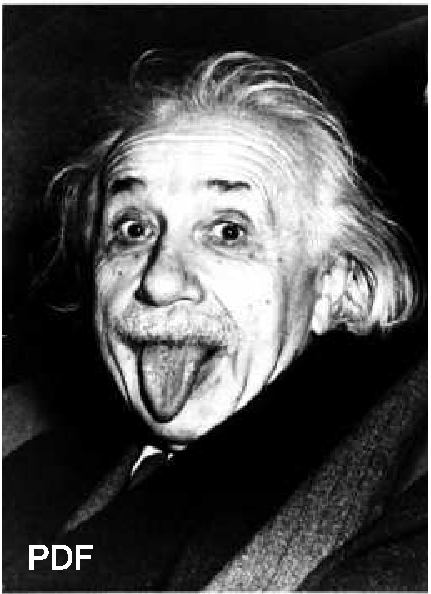
\includegraphics[width=0.6\textwidth]{einsteinlabel.pdf}
 \caption[Einstein-pdf]{Toller Typ. Das hier ist ein PDF (Vektorgrafik-f"ahiges Format).}
 \label{piceinsteinpdf}
\end{figure}

\begin{figure}[ht]
 \centering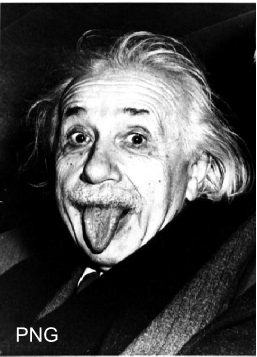
\includegraphics[width=0.6\textwidth]{einsteinlabel.png}
 \caption[Einstein-png]{Toller Typ. Das hier ist ein PNG (Bitmap-Format).}
 \label{piceinsteinpng}
\end{figure}

Wie binde ich ein Bild ein, das ich mit Matlabfrag erzeugt habe? (F�r eine genauere Erl�uterung zu Matlabfrag and Gnuplot schau Dir die Plauderstunde im Wiki zu diesem Thema an.)

\begin{figure}[ht]
 \centering
 \psfragfig[width=0.7\textwidth]{pics/APsMfrag}
 \caption[Aktionspotential]{Grafik erzeugt mit Psfrag (der Text in der Grafik wird durch die aktuelle LateX-Schriftart in der passenden Schriftgr��e ersetzt}
 \label{piceinsteinpng}
\end{figure}

\newpage\thispagestyle{empty}
\clearemptydoublepage


\chapter{Tabellen}
\label{Tabellen}
\thispagestyle{empty}

Wie erzeuge ich eine Tabelle ??

\vspace{5cm}

\begin{table}[h]
 \caption{Rechenvorteil der FFT gegen"uber der direkten FT}
 \begin{center}
 \begin{tabular}{|rrrr|}
 \hline
 & direkte FT & FFT & Rechenvorteil\\
 $N$ & $N^{2}$ & $N \log_{2} N$ & $\log_{2} N/N$ \\
 \hline
 \hline
   2&          4&        2&     50,0\%\\
   4&         16&        8&     50,0\%\\
   8&         64&       24&     37,5\%\\
  16&        256&       64&     25,0\%\\
  32&      1.024&      160&     15,6\%\\
  64&      4.096&      384&      9,4\%\\
 128&     16.384&      896&      5,5\%\\
 256&     65.536&    2.048&      3,1\%\\
 512&    262.144&    4.608&      1,8\%\\
1024&  1.048.576&   10.240&      1,0\%\\
2048&  4.194.304&   22.528&      0,5\%\\
4096& 16.777.216&   49.152&      0,3\%\\
8192& 67.108.864&  106.496&      0,2\%\\
 \hline
  \end{tabular}
 \end{center}
 \label{tablerechenvorteilfft}
\end{table}   

\newpage

Hier ist ein Beispiel f"ur eine colorierte Tabelle
\begin{table}[h!]
 \caption[Typische Verteilung der Ionen im Intra- und Extrazellul"arraum einer Muskelzelle.]{Typische Verteilung der Ionen im Intra- und Extrazellul"arraum einer Muskelzelle \cite{silbernagl01}. Durch den Konzentrationsunterschied entsteht f"ur jede Ionenart eine sogenannte Nernst-Spannung.}
\centering
\begin{tabular}{|>{\columncolor{hellblau}}c|c|c|c|}  
  \hline\rowcolor{hellblau}
  & intrazellul"are & exrazellul"are & Nernst-\\\rowcolor{hellblau}
   \, Ionenart\, &\, Konz. [$mmol/kg\,H_2O$]\, &\, Konz. [$mmol/kg\,H_2O$]\, &\, Spannung [mV]\, \\
  \hline \hline
  $K^{+}$&\cellcolor{hellgelb} 4,5 &\cellcolor{hellgelb} 160 &\cellcolor{hellgelb} -95,4\\
  $Na^{+}$&\cellcolor{hellgelb} 144 &\cellcolor{hellgelb} 7 &\cellcolor{hellgelb} 80,2\\
  $Ca^{2+}$&\cellcolor{hellgelb} 1,3 &\cellcolor{hellgelb} 0,00001-0,0001 &\cellcolor{hellgelb} 126,5-157,3\\
  $Cl^{-}$&\cellcolor{hellgelb} 114 &\cellcolor{hellgelb} 7 &\cellcolor{hellgelb} -74,5\\
  \hline
\end{tabular}
%  \label{ionenkonzentration}
 \vspace{2mm}
 \label{ionenkonzentration}
\end{table}


\newpage

In   diesem   Abschnitt   sollen lediglich   die   grundlegenden
Eigenschaften  der  Fouriertransformation kurz tabellarisch dargestellt werden
(Tabelle  \ref{tableeigenft}). Die  Beweise zu den Regeln und  alle  Eigenschaften
sind in \cite{gonzalez92bsp} zu finden.

\begin{table}[H]
 \begin{center}
  \begin{tabular}{|ccc|}
 \hline
 Ortsbereich &$\circ \hspace{-0.15cm} - \hspace{-0.15cm} \bullet$& Frequenzbereich\\\hline
 \hline
 Linearit"at &&  Linearit"at \\
 $k_{1}g(x)+k_{2}f(x)$ && $k_{1}G(u)+k_{2}F(u)$ \\\hline

 Symmetrie   &&  Symmetrie \\
 $F(x)$ && $f(-u)$ \\\hline

 Ortsskalierung && reziproke\\
 && Frequenzskalierung \\
 $f(kx)$ && $\frac{1}{|k|}F(\frac{u}{k})$\\\hline

 reziproke&&\\
 Ortsskalierung && Frequenzskalierung \\
 $\frac{1}{|k|}f(\frac{x}{k})$ && $F(ku)$\\\hline

 Ortsverschiebung && Phasenverschiebung \\
 $f(x-x_{0})$ && $F(u) e^{ -j 2 \pi u x_{0} }$\\\hline

 Modulation && Frequenzverschiebung \\
 $f(x) e^{ -j 2 \pi x u_{0} }$ && $F(u-u_{0})$\\\hline

 gerade Funktion && reelle Funktion \\
 $f_{g}(x)$ && $F_{g}(u)=R_{g}(u)$\\\hline

 ungerade Funktion && imagin"are Funktion \\
 $f_{u}(u)$ && $F_{u}(u)=jI_{u}(u)$\\\hline

 reelle Funktion && gerader Realteil,\\
 && ungerader Imagin"arteil \\
 $f(x)=f_{r}(u)$ && $F(u)=R_{g}(u)+j I_{u}(u)$\\\hline

 imagin"are Funktion && ungerader Realteil, \\
 && gerader Imagin"arteil \\
 $f(x)=j f_{i}(u)$ && $F(u)=R_{u}(u)+j I_{g}(u)$\\\hline

  \end{tabular}
 \end{center}
 \caption[Wichtige Eigenschaften der Fouriertransformation]{
Wichtige Eigenschaften der Fouriertransformation}
 \label{tableeigenft}
\end{table}

\newpage\thispagestyle{empty}
\clearemptydoublepage

\chapter{Formeln}
\label{formeln}
\thispagestyle{empty}

Viele, viele bunte Formeln....


\section{FFT-Algorithmus}

Am  Beispiel der 1D-DFT soll eine Variante des FFT-Algorithmus
an  dieser  Stelle  beschrieben werden: Basis-2-Algorithmus
mit Zerlegung im Zeitraum (engl. {\em decimation in time 
radix-2  algorithm}) \cite{gonzalez92bsp}.

 Zun"achst wird die Fouriertransformierte wie folgt umgeschrieben:
\begin{equation} 
 \label{eq21}
F(u) = \frac{1}{N} \sum \limits_{x=0}^{N-1}f(x) e^{ -j 2 \pi \frac{u x}{N} }
  = \frac{1}{N} \sum \limits_{x=0}^{N-1}f(x) W_{N}^{ux}
\textrm{,}
\end{equation}
\begin{equation}
\label{eq22}
\textrm{mit  }
  W_{N} = e^{ -j 2 \pi \frac{1}{N} }
\textrm{  und  $u=0,1,\dots,N-1$.}
\end{equation}

Unter  der Annahme, da"s $N$ eine Potenz zur Basis $2$ ist  und
$n$ und $L$ zur Menge der nat"urlichen Zahlen geh"oren, l"a"st sich
$N$ ausdr"ucken durch
\begin{equation}
\label{eq23}
N=2^{n}=2L
\textrm{.}
\end{equation}

Durch Substitution von Gl. \ref{eq23} in Gl. \ref{eq21} ergibt sich
\begin{eqnarray} 
\label{eq24}
F(u) &=& \frac{1}{2L} \sum \limits_{x=0}^{2L-1}f(x) W_{2L}^{ux} \nonumber \\
  &=& \frac{1}{2} \left [ \frac{1}{L} \sum \limits_{x=0}^{L-1}f(2x) W_{2L}^{u(2x)} +
     \frac{1}{L} \sum \limits_{x=0}^{L-1}f(2x+1) W_{2L}^{u(2x+1)} \right ]
\textrm{,}
\end{eqnarray}
und mit $W_{2L}^{2ux} = W_{L}^{ux}$ (aus Gl. \ref{eq22}) folgt schlie"slich
\begin{equation}
\label{eq25}
F(u) = \frac{1}{2} \left [ \frac{1}{L} \sum \limits_{x=0}^{L-1}f(2x) W_{L}^{ux}+
     \frac{1}{L} \sum \limits_{x=0}^{L-1}f(2x+1) W_{L}^{ux} W_{2L}^{u} \right ]
\textrm{.}
\end{equation}

In einem  n"achsten Schritt definiert man f"ur gerade und ungerade
Funk\-tions\-werte je eine Funktion $F(u)$
\begin{equation} 
\label{eq26}
F_{gerade}(u) = \frac{1}{L} \sum \limits_{x=0}^{L-1}f(2x) W_{L}^{ux} 
\textrm{ und}
\end{equation}
\begin{equation} 
\label{eq27}
F_{ungerade}(u) = \frac{1}{L} \sum \limits_{x=0}^{L-1}f(2x+1) W_{L}^{ux}
\textrm{ f"ur $u=0,1,\dots,L-1$.}
\end{equation}
Durch  Einsetzen  von Gl. \ref{eq26} und Gl. \ref{eq27}  reduziert  sich
Gl. \ref{eq25} zu
\begin{equation}
\label{eq28}
F(u) = \frac{1}{2} \left [ F_{gerade}(u) + F_{ungerade}(u) W_{2L}^{u} \right ]
\textrm{.}
\end{equation}
Mit $W_{L}^{u+L} = W_{L}^{u}$, $W_{2L}^{u+L} = -W_{2L}^{u}$ und den Gl.~\ref{eq25}
bis Gl.~\ref{eq28} ergibt sich
\begin{equation}
\label{eq29}
F(u+L) = \frac{1}{2} \left [ F_{gerade}(u) - F_{ungerade}(u) W_{2L}^{u} \right ]
\textrm{.}
\end{equation}

Somit  besteht  der  FFT-Algorithmus  in  der  sukzessiven
Anwendung  der Halbierung der diskreten Funktion $F(u)$.  Mit
Gl.  \ref{eq28} und Gl. \ref{eq29} liegen $N/2$-Punkt-Transformationen vor.
Diese  lassen  sich  wiederum in zwei Transformationen  der
halben  L"ange  aufteilen. Man erh"alt "ahnliche  Gleichungen,
nur  mit  dem Unterschied, da"s die Phasenverschiebung  sich
verdoppelt  hat.  Die  Halbierung mu"s konsequenterweise  f"ur  beide
Funktionen, gerade und ungerade, durchgef"uhrt werden.

Im letzten Schritt erh"alt man f"ur $\tilde{u}=0$ :
\begin{eqnarray}
F(0) &=& \frac{1}{2} \left [ \tilde{F}_{gerade}(0) + \tilde{F}_{ungerade}(0)
         W_{2\tilde{L}}^{0} \right ] \nonumber \\
     &=& f(0)+f(1)
\textrm{ und }\\
F(0+\tilde{L}) &=& F(1) = \frac{1}{2} \left [ \tilde{F}_{gerade}(0) - 
         \tilde{F}_{ungerade}(0) W_{2\tilde{L}}^{0} \right ] \nonumber \\
     &=& f(0)-f(1),
\end{eqnarray}
da $W=1$ und $\tilde{L}=1$ sind.

Am  Beispiel f"ur  $N=4$ soll dies demonstriert werden. Nach  Gl.~\ref{eq28}
und Gl.~\ref{eq29} erh"alt man ($L=2$)
\begin{eqnarray}
\label{eq210}
F(0) &=& \frac{1}{2} \left [ F_{gerade}(0) + F_{ungerade}(0) W_{4}^{0} \right ]
\textrm{,} \\
F(2) &=& \frac{1}{2} \left [ F_{gerade}(0) - F_{ungerade}(0) W_{4}^{0} \right ]
\textrm{,} \\
F(1) &=& \frac{1}{2} \left [ F_{gerade}(0) + F_{ungerade}(0) W_{4}^{1} \right ]
\textrm{,} \\
F(3) &=& \frac{1}{2} \left [ F_{gerade}(0) - F_{ungerade}(0) W_{4}^{1} \right ]
\label{eq211}
\textrm{.}
\end{eqnarray}
Mit Gl. \ref{eq22} gilt
\begin{equation}
  W_{4}^{0} = e^{ -j 2 \pi \frac{0}{4} } = 1
\textrm{ und }
  W_{4}^{1} = e^{ -j 2 \pi \frac{1}{4} } = -j
\textrm{.}
\end{equation}
Weiterhin nach \ref{eq26} und Gl. \ref{eq27}f"ur $u=0,1$
\begin{eqnarray}
F_{gerade}(0) &=& \frac{1}{2} \sum \limits_{x=0}^{1}f(2x) W_{2}^{0}  \nonumber \\
  &=& \frac{1}{2} \left [ f(0)W_{2}^{0} + f(2)W_{2}^{0} \right ]
  = \frac{1}{2} \left [ f(0) + f(2) \right ]
\textrm{,}\\
F_{ungerade}(0) &=& \frac{1}{2} \sum \limits_{x=0}^{1}f(2x+1) W_{2}^{0} \nonumber \\
  &=& \frac{1}{2} \left [ f(1)W_{2}^{0} + f(3)W_{2}^{0} \right ]
  = \frac{1}{2} \left [ f(1) + f(3) \right ]
\textrm{,}\\
F_{gerade}(1) &=& \frac{1}{2} \sum \limits_{x=0}^{1}f(2x) W_{2}^{x} \nonumber \\
  &=& \frac{1}{2} \left [ f(0)W_{2}^{0} + f(2)W_{2}^{1} \right ]
  = \frac{1}{2} \left [ f(0) - f(2) \right ]
\textrm{,}\\
F_{ungerade}(1) &=& \frac{1}{2} \sum \limits_{x=0}^{1}f(2x+1) W_{2}^{x} \nonumber \\
  &=& \frac{1}{2} \left [ f(1)W_{2}^{0} + f(3)W_{2}^{1} \right ]
  = \frac{1}{2} \left [ f(1) - f(3) \right ]
\textrm{,}
\end{eqnarray}
mit $W_{2}^{0} = 1$  und  $W_{2}^{1} = -1$.
Eingesetzt in Gl. \ref{eq210} bis Gl. \ref{eq211} folgt  das Ergebnis
\begin{eqnarray}
F(0) &=& \frac{1}{2} 
  \left \{ 
    \frac{1}{2} \left [ f(0) + f(2) \right ] + \frac{1}{2} \left [ f(1) + f(3) \right ]
  \right \} \nonumber \\
     &=& \frac{1}{4}
  \left \{ 
    \left [ f(0) + f(2) \right ] + \left [ f(1) + f(3) \right ]
  \right \}
\textrm{,}\\
F(2) &=& \frac{1}{2} 
  \left \{ 
    \frac{1}{2} \left [ f(0) + f(2) \right ] - \frac{1}{2} \left [ f(1) + f(3) \right ]
  \right \} \nonumber \\
     &=& \frac{1}{4}
  \left \{ 
    \left [ f(0) + f(2) \right ] - \left [ f(1) + f(3) \right ]
  \right \}
\textrm{,}\\
F(1) &=& \frac{1}{2} 
  \left \{ 
    \frac{1}{2} \left [ f(0) - f(2) \right ] + \frac{1}{2} \left [ f(1) - f(3) \right ] (-j)
  \right \} \nonumber \\
     &=& \frac{1}{4}
  \left \{ 
    \left [ f(0) - f(2) \right ] - j \left [ f(1) - f(3) \right ]
  \right \}
\textrm{,}\\
F(3) &=& \frac{1}{2} 
  \left \{ 
    \frac{1}{2} \left [ f(0) - f(2) \right ] - \frac{1}{2} \left [ f(1) - f(3) \right ] (-j)
  \right \} \nonumber \\
     &=& \frac{1}{4}
  \left \{ 
    \left [ f(0) - f(2) \right ] + j \left [ f(1) - f(3) \right ]
  \right \}
\textrm{.}
\end{eqnarray}

\newpage\thispagestyle{empty}
\clearemptydoublepage

\chapter{Zusammenfassung}
\label{zusammenfassung}
\thispagestyle{empty}


\newpage\thispagestyle{empty}
\clearemptydoublepage

\chapter{Ausblick}
\label{ausblick}
\thispagestyle{empty}


\newpage\thispagestyle{empty}
\clearemptydoublepage

\begin{appendix}
\chapter{Anhang1}
\label{anhang1}
\thispagestyle{empty}

\end{appendix}



%%%%%%%%%%%%%%%%%%%%%%%%%%%%%%%%%%%%%%%%%%%%%%%%%%%%%%%
\backmatter %%%%%%%%%%%%%%%%%%%%%%%%%%%%%%%%%%%%%%%%%%%%%
%%%%%%%%%%%%%%%%%%%%%%%%%%%%%%%%%%%%%%%%%%%%%%%%%%%%%%%

\listoffigures
\newpage\thispagestyle{empty}
\clearemptydoublepage

\listoftables
\newpage\thispagestyle{empty}
\clearemptydoublepage


%%%%%%%%%%%%%%%%%%%%%%
% Citation / Reference Style  %
%%%%%%%%%%%%%%%%%%%%%%
\ifapa
	\bibliographystyle{styles/natdinIBT} 				% APA style in alphabetical order
\else
	\ifenglish
		\bibliographystyle{styles/dipl}						% IEEE style, English Version
	\else
		\bibliographystyle{styles/diplGerman}			% IEEE style, German Version 
	\fi
\fi

\bibliography{literatur,refbase}
\thispagestyle{empty}
\cleardoublepage

\ifthesisisdiss
	\chapter*{List of Publications and Supervised Thesis}
% The next line is important, such that the text in the header cotains the correct text. If you do not include this line the header text will be the same as in the previous chapter, as the \chapter* command does not alter the header.
\markboth{List of Publications and Supervised Thesis}{List of Publications and Supervised Thesis}
\label{sec:Publications}
% The next line adds the chapter to the table of contents, as the \chapter* command does not alter the toc. 
\addcontentsline{toc}{chapter}{List of Publications and Supervised Thesis}

\section*{Journal Articles}
\label{sec:PublicationsJournal}

\begin{itemize}
	\item \textbf{Your Name}, other authors, and O. D\"ossel, \textit{title}, Journal, Issue, Pages, Year
\end{itemize}

\section*{Book Chapters}
%\sectionmark{Book Chapters}
\label{sec:Books}

\begin{itemize}
	\item 
\end{itemize}


\section*{Refereed Conference Articles}
\label{sec:PublicationsConferences}

\begin{itemize}
	\item 
\end{itemize}

\section*{Refereed Conference Abstracts}
\label{sec:PublicationsPresentations}

\begin{itemize}
	\item 
\end{itemize}


\section*{Conference Presentations}

\begin{itemize}
	\item 
\end{itemize}


\section*{Reports and Theses}
\label{sec:PublicationsReports}

\begin{itemize}
	\item 
	\item \textbf{your name}, \textit{title}, Diplomarbeit, Universit\"at Karlsruhe (TH), Karlsruhe, 2008
	\item \textbf{your name}, \textit{title}, Studienarbeit, Universit\"at Karlsruhe, Institute of Biomedical Engineering, 2007
\end{itemize}


\section*{Supervised Student Theses}
\label{sec:PublicationsSupervisor}

\begin{itemize}
	\item student name, \textit{title}, Diplomarbeit, Institute of Biomedical Engineering, Karlsruhe Institute of Technology (KIT), Karlsruhe, year
\end{itemize}


\section*{Awards \& Grants}
\label{sec:CVawardsGrants}

\begin{itemize}
	\item 
\end{itemize}

	\newpage\thispagestyle{empty}
	\clearemptydoublepage
\fi

\end{document}
